\documentclass{article}
\usepackage{setspace}
\usepackage[utf8]{inputenc}
\usepackage{natbib}
\usepackage{url}

\usepackage{graphicx}
\graphicspath{ {figures/} }

\title{Text Analysis of \emph{Hamilton}}
\author{Nathan Schor}
\date{March 13, 2022}

\doublespacing
\begin{document}

\maketitle
\tableofcontents
\listoffigures

\section{Introduction}

The purpose of this research is to investigate the role of different sets of stop words and tokenization schemes in natural language processing (NLP) applied to the lyrics of the musical \emph{Hamilton}. We experiment with how four different sources of stop words and tokenizing at the word vs. sentence level affects sentiment analysis, term frequency-inverse document frequency (\emph{tf-idf}), topic modeling, and a chat bot. We begin by examining how sentiment changes throughout the musical and which pair of songs has the largest shift in sentiment. Next, we use \emph{tf-idf} to identify the most important word for each speaker. After, we see if the topic model is able to identify the speaker based on their words. Lastly, we develop a chat bot that is able to answer questions on a corpus that contains \emph{Hamilton's} wikipedia page augmented with results from this analysis. 

Using \cite{Silge2022}




\section{Literature Review}

\section{Data}

The main dataset is obtained from the website \cite{Kaggle2019}. It contains the entirety of the musical in a csv file with 3,634 rows and 3 columns. The \emph{lines} column gives the line that is spoken. The \emph{speaker} column gives the names of the people speaking (can be more than one character singing at the same time). \emph{Title} gives the name of the song. 5 random rows of the data are shown in \ref{tab:example}. The main corpus for the chat bot is \cite{Wiki}.

\begin{table}
\caption{Example of the \emph{Hamilton} dataset.}
\label{tab:example}

\begin{tabular}{r|l|l|l}
\hline
entry & title & speaker & lines\\
\hline
1 & The Election of 1800 & JEFFERSON & 'cuz I'm the President. Hey, Burr, when you see Hamilton, thank him for the endorsement\\
\hline
2 & Blow Us All Away & PHILIP & I came to ask you for advice. This is my very first duel\\
\hline
3 & It's Quiet Uptown & HAMILTON & I take the children to church on Sunday\\
\hline
4 & Satisfied & ANGELICA & Have to be na<ef>ve to set that aside\\
\hline
5 & Right Hand Man & WASHINGTON & But the elephant is in the room\\
\hline
\end{tabular}

\end{table}

\subsection{Stop Words}
Three sources are used to obtain the list of stop words. They are the SMART lexicon from \cite{Lewis2004}, snowball from \cite{snowball}, and onix.

\subsection{Sentiment}

Three lexicons are used to obtain sentiment. They are the AFINN dataset from \cite{nielsen11}, the nrc dataset from INSERT HERE, and the bing dataset from INSERT HERE.

AFINN assigns words an integer value in $\{-5, -4, ..., 4, 5\}$ with -5 having the most negative sentiment and 5 having the most positive sentiment. Swear words/insults have -5, words like "superb" or "breathtaking" are 5, and "some kind" is 0. There are 2,477 terms. 

nrc assigns each of its 13,875 words to 1 of 8 emotional categories. For the purpose of this analysis, only words in the "positive" or "negative" emotion category are retained. 






\section{Research Design and Modeling Methods}

\section{Results}

\begin{figure}[h]
    \caption{Sentiment Analysis by preprocessing group. \label{fig:sentiment}}
    \centering
    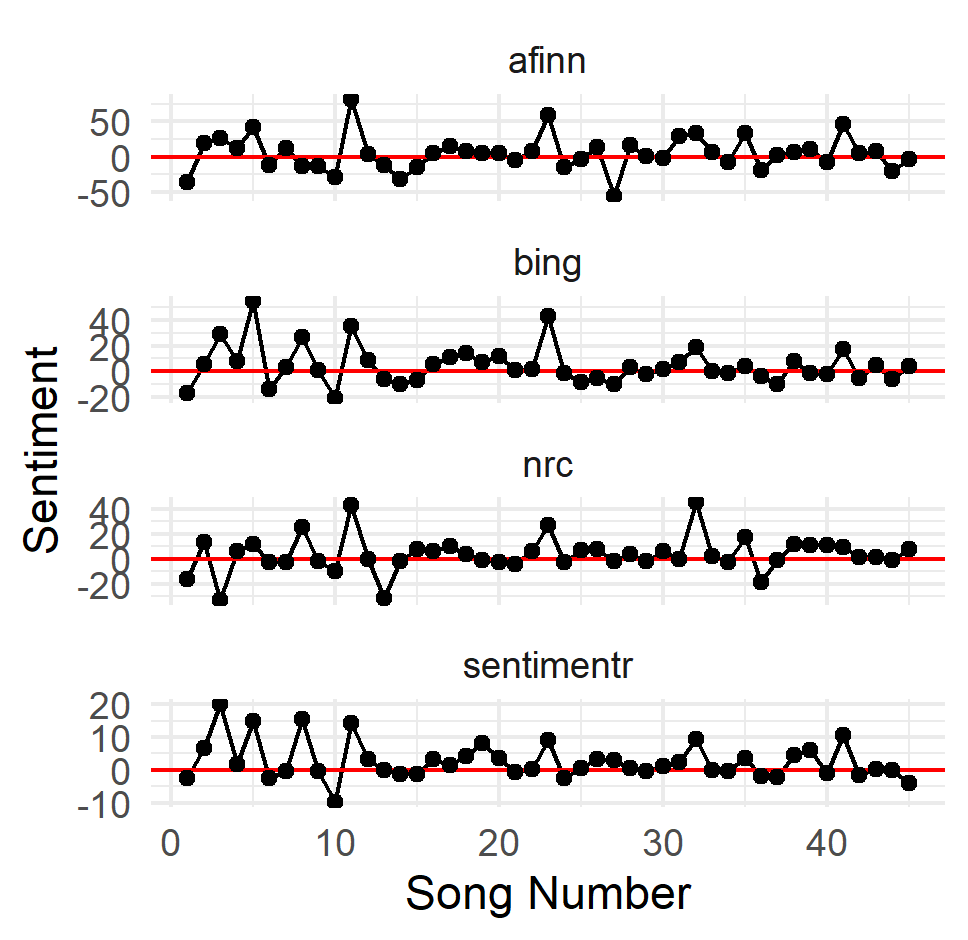
\includegraphics[width=0.2\paperwidth]{sentiment_by_stopwords.png}
\end{figure}



\section{Analysis and Interpretation}

\begin{table}
\caption{tf-idf by character}
\label{tab:tfidf}

\begin{tabular}{r|l|l|l|l|l|l}
\hline
\textbf{Entry} & \textbf{Speaker} & \textbf{SMART} & \textbf{snowball} & \textbf{onix} & \textbf{All Lexicons} & \textbf{All Words}\\
\hline
1 & Angelica & satisfied & satisfied & satisfied & satisfied & satisfied\\
\hline
2 & Burr & room & room & immigrant & immigrant & room\\
\hline
3 & Company & number & number & aaaah & aaaah & number\\
\hline
4 & Eliza & huit & enough & look & huit & enough\\
\hline
5 & Eliza & huit & enough & look & sept & enough\\
\hline
6 & Ensemble & buck & buck & buck & buck & buck\\
\hline
7 & Hamilton & sir & sir & sir & sir & i\\
\hline
8 & Jefferson & what'd & what'd & what'd & what'd & what'd\\
\hline
9 & Lafayette & onarchy & onarchy & onarchy & onarchy & onarchy\\
\hline
10 & Lafayette & onarchy & onarchy & onarchy & onarchy & oui\\
\hline
11 & Laurens & colonies & colonies & colonies & colonies & colonies\\
\hline
12 & Lee & crisis & crisis & crisis & crisis & crisis\\
\hline
13 & Madison & size & size & size & size & size\\
\hline
14 & Maria & sir & yes & yes & sir & yes\\
\hline
15 & Men & satisfied & satisfied & satisfied & satisfied & satisfied\\
\hline
16 & Mulligan & hercules & hercules & hercules & hercules & hercules\\
\hline
17 & Mulligan & hercules & hercules & hercules & hercules & lovin\\
\hline
18 & Philip & deux & deux & deux & deux & deux\\
\hline
19 & Philip & deux & deux & deux & deux & huit\\
\hline
20 & Seabury & heed & heed & heed & heed & heed\\
\hline
21 & Seabury & heed & heed & heed & heed & interests\\
\hline
22 & Washington & goodbye & goodbye & goodbye & goodbye & goodbye\\
\hline
23 & Women & helpless & helpless & helpless & helpless & helpless\\
\hline
\end{tabular}

\end{table}

\section{Conclusions}

\bibliography{references}
\bibliographystyle{apalike}


\end{document}